\documentclass[]{article}
\usepackage{lmodern}
\usepackage{amssymb,amsmath}
\usepackage{ifxetex,ifluatex}
\usepackage{fixltx2e} % provides \textsubscript
\ifnum 0\ifxetex 1\fi\ifluatex 1\fi=0 % if pdftex
  \usepackage[T1]{fontenc}
  \usepackage[utf8]{inputenc}
\else % if luatex or xelatex
  \ifxetex
    \usepackage{mathspec}
  \else
    \usepackage{fontspec}
  \fi
  \defaultfontfeatures{Ligatures=TeX,Scale=MatchLowercase}
\fi
% use upquote if available, for straight quotes in verbatim environments
\IfFileExists{upquote.sty}{\usepackage{upquote}}{}
% use microtype if available
\IfFileExists{microtype.sty}{%
\usepackage{microtype}
\UseMicrotypeSet[protrusion]{basicmath} % disable protrusion for tt fonts
}{}
\usepackage[margin=1in]{geometry}
\usepackage{hyperref}
\hypersetup{unicode=true,
            pdftitle={Videogrammetry Metrics for Assessing Fish Foraging Behavior: Implications for Behavioral Ecology and Management},
            pdfauthor={Keane Flynn},
            pdfborder={0 0 0},
            breaklinks=true}
\urlstyle{same}  % don't use monospace font for urls
\usepackage{color}
\usepackage{fancyvrb}
\newcommand{\VerbBar}{|}
\newcommand{\VERB}{\Verb[commandchars=\\\{\}]}
\DefineVerbatimEnvironment{Highlighting}{Verbatim}{commandchars=\\\{\}}
% Add ',fontsize=\small' for more characters per line
\usepackage{framed}
\definecolor{shadecolor}{RGB}{248,248,248}
\newenvironment{Shaded}{\begin{snugshade}}{\end{snugshade}}
\newcommand{\KeywordTok}[1]{\textcolor[rgb]{0.13,0.29,0.53}{\textbf{#1}}}
\newcommand{\DataTypeTok}[1]{\textcolor[rgb]{0.13,0.29,0.53}{#1}}
\newcommand{\DecValTok}[1]{\textcolor[rgb]{0.00,0.00,0.81}{#1}}
\newcommand{\BaseNTok}[1]{\textcolor[rgb]{0.00,0.00,0.81}{#1}}
\newcommand{\FloatTok}[1]{\textcolor[rgb]{0.00,0.00,0.81}{#1}}
\newcommand{\ConstantTok}[1]{\textcolor[rgb]{0.00,0.00,0.00}{#1}}
\newcommand{\CharTok}[1]{\textcolor[rgb]{0.31,0.60,0.02}{#1}}
\newcommand{\SpecialCharTok}[1]{\textcolor[rgb]{0.00,0.00,0.00}{#1}}
\newcommand{\StringTok}[1]{\textcolor[rgb]{0.31,0.60,0.02}{#1}}
\newcommand{\VerbatimStringTok}[1]{\textcolor[rgb]{0.31,0.60,0.02}{#1}}
\newcommand{\SpecialStringTok}[1]{\textcolor[rgb]{0.31,0.60,0.02}{#1}}
\newcommand{\ImportTok}[1]{#1}
\newcommand{\CommentTok}[1]{\textcolor[rgb]{0.56,0.35,0.01}{\textit{#1}}}
\newcommand{\DocumentationTok}[1]{\textcolor[rgb]{0.56,0.35,0.01}{\textbf{\textit{#1}}}}
\newcommand{\AnnotationTok}[1]{\textcolor[rgb]{0.56,0.35,0.01}{\textbf{\textit{#1}}}}
\newcommand{\CommentVarTok}[1]{\textcolor[rgb]{0.56,0.35,0.01}{\textbf{\textit{#1}}}}
\newcommand{\OtherTok}[1]{\textcolor[rgb]{0.56,0.35,0.01}{#1}}
\newcommand{\FunctionTok}[1]{\textcolor[rgb]{0.00,0.00,0.00}{#1}}
\newcommand{\VariableTok}[1]{\textcolor[rgb]{0.00,0.00,0.00}{#1}}
\newcommand{\ControlFlowTok}[1]{\textcolor[rgb]{0.13,0.29,0.53}{\textbf{#1}}}
\newcommand{\OperatorTok}[1]{\textcolor[rgb]{0.81,0.36,0.00}{\textbf{#1}}}
\newcommand{\BuiltInTok}[1]{#1}
\newcommand{\ExtensionTok}[1]{#1}
\newcommand{\PreprocessorTok}[1]{\textcolor[rgb]{0.56,0.35,0.01}{\textit{#1}}}
\newcommand{\AttributeTok}[1]{\textcolor[rgb]{0.77,0.63,0.00}{#1}}
\newcommand{\RegionMarkerTok}[1]{#1}
\newcommand{\InformationTok}[1]{\textcolor[rgb]{0.56,0.35,0.01}{\textbf{\textit{#1}}}}
\newcommand{\WarningTok}[1]{\textcolor[rgb]{0.56,0.35,0.01}{\textbf{\textit{#1}}}}
\newcommand{\AlertTok}[1]{\textcolor[rgb]{0.94,0.16,0.16}{#1}}
\newcommand{\ErrorTok}[1]{\textcolor[rgb]{0.64,0.00,0.00}{\textbf{#1}}}
\newcommand{\NormalTok}[1]{#1}
\usepackage{graphicx,grffile}
\makeatletter
\def\maxwidth{\ifdim\Gin@nat@width>\linewidth\linewidth\else\Gin@nat@width\fi}
\def\maxheight{\ifdim\Gin@nat@height>\textheight\textheight\else\Gin@nat@height\fi}
\makeatother
% Scale images if necessary, so that they will not overflow the page
% margins by default, and it is still possible to overwrite the defaults
% using explicit options in \includegraphics[width, height, ...]{}
\setkeys{Gin}{width=\maxwidth,height=\maxheight,keepaspectratio}
\IfFileExists{parskip.sty}{%
\usepackage{parskip}
}{% else
\setlength{\parindent}{0pt}
\setlength{\parskip}{6pt plus 2pt minus 1pt}
}
\setlength{\emergencystretch}{3em}  % prevent overfull lines
\providecommand{\tightlist}{%
  \setlength{\itemsep}{0pt}\setlength{\parskip}{0pt}}
\setcounter{secnumdepth}{0}
% Redefines (sub)paragraphs to behave more like sections
\ifx\paragraph\undefined\else
\let\oldparagraph\paragraph
\renewcommand{\paragraph}[1]{\oldparagraph{#1}\mbox{}}
\fi
\ifx\subparagraph\undefined\else
\let\oldsubparagraph\subparagraph
\renewcommand{\subparagraph}[1]{\oldsubparagraph{#1}\mbox{}}
\fi

%%% Use protect on footnotes to avoid problems with footnotes in titles
\let\rmarkdownfootnote\footnote%
\def\footnote{\protect\rmarkdownfootnote}

%%% Change title format to be more compact
\usepackage{titling}

% Create subtitle command for use in maketitle
\newcommand{\subtitle}[1]{
  \posttitle{
    \begin{center}\large#1\end{center}
    }
}

\setlength{\droptitle}{-2em}

  \title{Videogrammetry Metrics for Assessing Fish Foraging Behavior:
Implications for Behavioral Ecology and Management}
    \pretitle{\vspace{\droptitle}\centering\huge}
  \posttitle{\par}
    \author{Keane Flynn}
    \preauthor{\centering\large\emph}
  \postauthor{\par}
      \predate{\centering\large\emph}
  \postdate{\par}
    \date{4/30/2019}


\begin{document}
\maketitle

\section{\texorpdfstring{\textbf{Introduction}}{Introduction}}\label{introduction}

\begin{verbatim}
Fish foraging behavior has long been a topic of natural observation, wonder, and recreational curiosity (Walton 1655). In recent years, this area of observation has extended beyond the realm as an enigmatic phenomenon and taken its place as a series of qualitative metrics in fisheries ecology. But with recent advances in computer technologies and programming languages, we are capable of extending these qualitatives behavioral metrics into quantitative values which can be further mathematically and statistically analyzed to show distinct differences in behavior. These differences in foraging behaviors have been shown to be linked to changes in physical habitat characteristics that might be indicative of decreasing habitat quality for foraging fish (Rossi et al. 2019 in prep; Steingrímmson 2012; Fausch et al. 1997). 
Using the three dimensional videogrammetric program VidSync, quantifying previously generalized qualitative/quantitative values has become a relatively easy process that has the potential to offer results with more statistical significance than previous behavioral observation methods (Neuswanger 2014). This method makes use of two underwater cameras mounted in a fixed location relative to one another recording simultaneous video of fish behavior. Doing so allows for an almost entirely non-invasive way to record fish behavior, whereas many current methods rely on snorkel observations. Once the videos have been processed, an   X, Y, Z coordinate, a timecode, and a behavioral observation type are assigned to each point created for the video sample in the program. These coordinates, timecodes, and observations can then be exported and processed into code-based programs to create statistical and graphical representations of the data collected.
This program offers a number of advantages to traditional fish foraging observations, the largest of which being ease of quantifying spatial habitat use metrics within sub-millimeter accuracy, which will be expanded upon in the methods section. Additionally, this method of observation allows to expand forage observations beyond focal animal sampling, which has been the most common method for recording fish behavior in natural experiments, to other methods of behavior sampling methods such as sampling all occurrences of behaviors, sequence sampling, and scan sampling (Altmann 1974). While previous field observation methods could only account for one of these observation methods based on physical restrictions, replayable video allows for a higher confidence in behavioral observation assignment. Being able to track multiple individuals throughout a video sample allows for a complete assessment of behavioural observations for all individuals in the sample, hence creating a larger sample size for improved statistical analysis.
In previous research, these estimations of distances travelled, area of habitat, size of subjects, specific foraging patches, etc. conducted during snorkel surveys were capable of assigning numeric values to these metrics, but with a higher degree of uncertainty (Nakano et al. 1999; Nielsen 1992; Steingrímsson & Grant 2008). While some of these methods have proved useful for changes in habitat usage, these methods are inherently based on location estimations and lack critical pieces of information for properly classifying habitat use. The issue with these previously used methods is that the metrics for habitat use is generally two-dimensional, which disregards many phenomenon such as physical habitat characteristics and location of prey input that might affect location of fish along the Z-axis (Figure 1).
\end{verbatim}

\begin{figure}
\centering
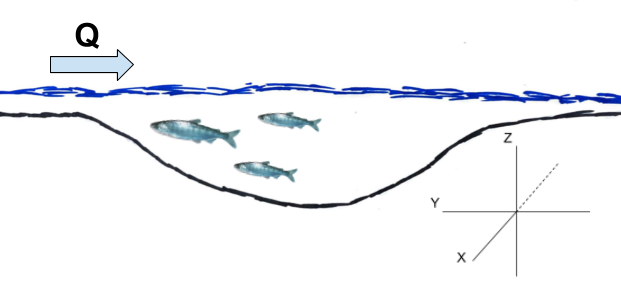
\includegraphics{XYZPlanes.png}
\caption{\textbf{Figure 1} \emph{Profile view of a pool-riffle sequence
with X, Y, Z planes relative to a fish maintaining positive rheotaxis.}}
\end{figure}

\begin{verbatim}
We hope to address some of the potential uses of these methods, but also realize that there are situations in which it might not be in the best interest to use these methods: they involve more post-capture editing and analyzation than that of snorkel observations, plotting movement movement points and territories can be more complex than doing so using the animal movement extension in ArcView (Hooge & Eichenlaub 2000). Given the resources to use this method are available, we find that it has many attributes that make up for the shortcomings of previously used methods. In this paper, we will elaborate upon the metrics that can be accurately derived using VidSync and the ecological implications of each. 
\end{verbatim}

\subsection{Load Libraries}\label{load-libraries}

\section{Importing VidSync CSV File}\label{importing-vidsync-csv-file}

\begin{Shaded}
\begin{Highlighting}[]
\NormalTok{VidSync_Test_Data <-}\StringTok{ }\NormalTok{readr}\OperatorTok{::}\KeywordTok{read_csv}\NormalTok{(}\DataTypeTok{file =} \StringTok{"Porter_BACI_RoachRun_5July2018_Part1.csv"}\NormalTok{, }
                             \DataTypeTok{skip =} \DecValTok{2}\NormalTok{,}
                             \DataTypeTok{col_names =} \KeywordTok{c}\NormalTok{(}\StringTok{"objects"}\NormalTok{, }\StringTok{"event"}\NormalTok{, }\StringTok{"timecode"}\NormalTok{, }\StringTok{"time_sec"}\NormalTok{, }\StringTok{"X"}\NormalTok{, }\StringTok{"Y"}\NormalTok{, }\StringTok{"Z"}\NormalTok{, }\StringTok{"pld_error"}\NormalTok{, }\StringTok{"projection_error"}\NormalTok{, }\StringTok{"nearest_camera_distance"}\NormalTok{, }\StringTok{"screen_coordinates"}\NormalTok{),}
                    \DataTypeTok{col_types =} \StringTok{"cccdddddddd"}\NormalTok{) }\OperatorTok\StringTok{ }
\StringTok{  }\KeywordTok{mutate}\NormalTok{(}\DataTypeTok{subsample =} \KeywordTok{as.numeric}\NormalTok{(}\KeywordTok{str_extract}\NormalTok{(objects, }\StringTok{"}\CharTok{\textbackslash{}\textbackslash{}}\StringTok{d"}\NormalTok{))) }\OperatorTok
\StringTok{  }\KeywordTok{mutate}\NormalTok{(}\DataTypeTok{fish_ID =} \KeywordTok{as.numeric}\NormalTok{(}\KeywordTok{str_extract}\NormalTok{(objects, }\StringTok{"}\CharTok{\textbackslash{}\textbackslash{}}\StringTok{h}\CharTok{\textbackslash{}\textbackslash{}}\StringTok{d\{1,2\}"}\NormalTok{))) }\OperatorTok
\StringTok{  }\KeywordTok{mutate}\NormalTok{(}\DataTypeTok{species =} \KeywordTok{str_extract}\NormalTok{(objects, }\StringTok{"Omykiss|Okisutch"}\NormalTok{)) }\OperatorTok\StringTok{ }\CommentTok{#Note that the use of regular expressions in this line are to be specified to whatever species are recorded in your experiment}
\StringTok{  }\KeywordTok{select}\NormalTok{(subsample, fish_ID, species, time_sec, X, Y, Z, objects, event) }\CommentTok{#All other data vectors were excluded for the sake of neatness and what is useful in the metrics below}
\end{Highlighting}
\end{Shaded}

\begin{verbatim}
## Warning in rbind(names(probs), probs_f): number of columns of result is not
## a multiple of vector length (arg 1)
\end{verbatim}

\begin{verbatim}
## Warning: 475 parsing failures.
## row # A tibble: 5 x 5 col     row col   expected   actual     file                                   expected   <int> <chr> <chr>      <chr>      <chr>                                  actual 1     1 <NA>  11 columns 10 columns 'Porter_BACI_RoachRun_5July2018_Part1~ file 2     2 <NA>  11 columns 10 columns 'Porter_BACI_RoachRun_5July2018_Part1~ row 3     3 <NA>  11 columns 10 columns 'Porter_BACI_RoachRun_5July2018_Part1~ col 4     4 <NA>  11 columns 10 columns 'Porter_BACI_RoachRun_5July2018_Part1~ expected 5     5 <NA>  11 columns 10 columns 'Porter_BACI_RoachRun_5July2018_Part1~
## ... ................. ... .......................................................................... ........ .......................................................................... ...... .......................................................................... .... .......................................................................... ... .......................................................................... ... .......................................................................... ........ ..........................................................................
## See problems(...) for more details.
\end{verbatim}

\section{Nearest Neighbor Distance
(NND)}\label{nearest-neighbor-distance-nnd}

NND is calculated by finding the nearest neighbor to each unique fish
over the course of a subsample. The final NND column will represent the
closest nearest neighbor for each fish and exclude any larger distances
(in cm) so as to not skew the data away from any values that are the
absolute nearest neighbor point over the course of the subsample. It is
important to note that subsamples with only one observed fish will
produce an NND that is infinite and should be dealt with accordingly
when graphing/calculating statistics on these values.

\begin{Shaded}
\begin{Highlighting}[]
\NormalTok{NND_Data <-}\StringTok{ }\NormalTok{VidSync_Test_Data }\OperatorTok\StringTok{ }
\StringTok{  }\KeywordTok{filter}\NormalTok{(}\KeywordTok{grepl}\NormalTok{(}\StringTok{"^Subsample.*"}\NormalTok{, objects)) }\OperatorTok
\StringTok{  }\KeywordTok{filter}\NormalTok{(}\OperatorTok{!}\KeywordTok{grepl}\NormalTok{(}\StringTok{"^Length.*"}\NormalTok{, event)) }\OperatorTok
\StringTok{  }\KeywordTok{filter}\NormalTok{(}\OperatorTok{!}\KeywordTok{grepl}\NormalTok{(}\StringTok{"^Attack.*"}\NormalTok{, event)) }\OperatorTok
\StringTok{  }\KeywordTok{filter}\NormalTok{(}\OperatorTok{!}\KeywordTok{grepl}\NormalTok{(}\StringTok{"^Nip.*"}\NormalTok{, event)) }\OperatorTok
\StringTok{  }\KeywordTok{na.omit}\NormalTok{() }\OperatorTok\StringTok{ }\CommentTok{#To remove any additional rows from the data set not associated with fish (i.e. surface shots)}
\StringTok{  }\KeywordTok{arrange}\NormalTok{(time_sec) }\OperatorTok
\StringTok{  }\KeywordTok{group_by}\NormalTok{(time_sec) }\OperatorTok
\StringTok{  }\KeywordTok{mutate}\NormalTok{(}\DataTypeTok{distance_between_X =}\NormalTok{ X }\OperatorTok{-}\StringTok{ }\KeywordTok{lag}\NormalTok{(X, }\DataTypeTok{default =} \KeywordTok{first}\NormalTok{(X))) }\OperatorTok
\StringTok{  }\KeywordTok{mutate}\NormalTok{(}\DataTypeTok{distance_between_Y =}\NormalTok{ Y }\OperatorTok{-}\StringTok{ }\KeywordTok{lag}\NormalTok{(Y, }\DataTypeTok{default =} \KeywordTok{first}\NormalTok{(Y))) }\OperatorTok
\StringTok{  }\KeywordTok{mutate}\NormalTok{(}\DataTypeTok{distance_between_Z =}\NormalTok{ Z }\OperatorTok{-}\StringTok{ }\KeywordTok{lag}\NormalTok{(Z, }\DataTypeTok{default =} \KeywordTok{first}\NormalTok{(Z))) }\OperatorTok
\StringTok{  }\KeywordTok{mutate}\NormalTok{(}\DataTypeTok{nnd_cm =} \KeywordTok{sqrt}\NormalTok{((distance_between_X)}\OperatorTok{^}\DecValTok{2} \OperatorTok{+}\StringTok{ }
\StringTok{                      }\NormalTok{(distance_between_Y)}\OperatorTok{^}\DecValTok{2} \OperatorTok{+}
\StringTok{                      }\NormalTok{(distance_between_Z)}\OperatorTok{^}\DecValTok{2}\NormalTok{)) }\OperatorTok
\StringTok{  }\KeywordTok{group_by}\NormalTok{(time_sec) }\OperatorTok
\StringTok{  }\KeywordTok{filter}\NormalTok{(}\OperatorTok{!}\NormalTok{nnd_cm }\OperatorTok{==}\StringTok{ }\DecValTok{0}\NormalTok{) }\OperatorTok
\StringTok{  }\KeywordTok{filter}\NormalTok{(nnd_cm }\OperatorTok{==}\StringTok{ }\KeywordTok{min}\NormalTok{(nnd_cm)) }\OperatorTok
\StringTok{  }\KeywordTok{ungroup}\NormalTok{() }\OperatorTok\StringTok{ }
\StringTok{  }\KeywordTok{distinct}\NormalTok{(fish_ID, }\DataTypeTok{.keep_all =} \OtherTok{TRUE}\NormalTok{) }\OperatorTok\StringTok{ }
\StringTok{  }\KeywordTok{arrange}\NormalTok{(subsample, fish_ID, time_sec) }\OperatorTok
\StringTok{  }\KeywordTok{select}\NormalTok{(subsample, fish_ID, time_sec, nnd_cm) }
\end{Highlighting}
\end{Shaded}

\section{Distance per Time}\label{distance-per-time}

\begin{Shaded}
\begin{Highlighting}[]
\NormalTok{DistancePerTime_Data <-}\StringTok{ }\NormalTok{VidSync_Test_Data }\OperatorTok\StringTok{ }
\StringTok{  }\KeywordTok{filter}\NormalTok{(}\OperatorTok{!}\KeywordTok{grepl}\NormalTok{(}\StringTok{"Surface_Shots.*"}\NormalTok{, objects)) }\OperatorTok
\StringTok{  }\KeywordTok{filter}\NormalTok{(}\OperatorTok{!}\KeywordTok{grepl}\NormalTok{(}\StringTok{"^Length.*"}\NormalTok{, event)) }\OperatorTok
\StringTok{  }\KeywordTok{group_by}\NormalTok{(fish_ID) }\OperatorTok\StringTok{ }
\StringTok{  }\KeywordTok{mutate}\NormalTok{(}\DataTypeTok{distance_travelled_X_cm =}\NormalTok{ X }\OperatorTok{-}\StringTok{ }\KeywordTok{lag}\NormalTok{(X, }\DataTypeTok{default =} \KeywordTok{first}\NormalTok{(X))) }\OperatorTok
\StringTok{  }\KeywordTok{mutate}\NormalTok{(}\DataTypeTok{distance_travelled_Y_cm =}\NormalTok{ Y }\OperatorTok{-}\StringTok{ }\KeywordTok{lag}\NormalTok{(Y, }\DataTypeTok{default =} \KeywordTok{first}\NormalTok{(Y))) }\OperatorTok
\StringTok{  }\KeywordTok{mutate}\NormalTok{(}\DataTypeTok{distance_travelled_Z_cm =}\NormalTok{ Z }\OperatorTok{-}\StringTok{ }\KeywordTok{lag}\NormalTok{(Z, }\DataTypeTok{default =} \KeywordTok{first}\NormalTok{(Z))) }\OperatorTok
\StringTok{  }\KeywordTok{mutate}\NormalTok{(}\DataTypeTok{fish_distance_travelled_cm =} \KeywordTok{sqrt}\NormalTok{((distance_travelled_X_cm)}\OperatorTok{^}\DecValTok{2}
                                        \OperatorTok{+}\StringTok{ }\NormalTok{(distance_travelled_Y_cm)}\OperatorTok{^}\DecValTok{2}
                                        \OperatorTok{+}\StringTok{ }\NormalTok{(distance_travelled_Z_cm)}\OperatorTok{^}\DecValTok{2}\NormalTok{)) }\OperatorTok
\StringTok{  }\KeywordTok{ungroup}\NormalTok{() }\OperatorTok\StringTok{ }
\StringTok{  }\KeywordTok{group_by}\NormalTok{(fish_ID) }\OperatorTok
\StringTok{  }\KeywordTok{mutate}\NormalTok{(}\DataTypeTok{distance_cm_per_sec =}\NormalTok{ fish_distance_travelled_cm }\OperatorTok{/}\NormalTok{(time_sec }\OperatorTok{-}\StringTok{ }\KeywordTok{lag}\NormalTok{(time_sec, }\DataTypeTok{default =} \KeywordTok{first}\NormalTok{(time_sec)))) }\OperatorTok
\StringTok{  }\KeywordTok{filter}\NormalTok{(}\OperatorTok{!}\NormalTok{distance_cm_per_sec }\OperatorTok{==}\StringTok{ }\OtherTok{Inf}\NormalTok{) }\OperatorTok\StringTok{ }
\StringTok{  }\KeywordTok{arrange}\NormalTok{(subsample, fish_ID, time_sec) }\OperatorTok
\StringTok{  }\KeywordTok{select}\NormalTok{(subsample, fish_ID, time_sec, distance_cm_per_sec)}
\end{Highlighting}
\end{Shaded}

\section{Proportion of Forage
Behaviors}\label{proportion-of-forage-behaviors}

\begin{Shaded}
\begin{Highlighting}[]
\NormalTok{ForageBehaviors_Data <-}\StringTok{ }\NormalTok{VidSync_Test_Data }\OperatorTok\StringTok{ }
\StringTok{  }\KeywordTok{filter}\NormalTok{(}\OperatorTok{!}\KeywordTok{grepl}\NormalTok{(}\StringTok{"Surface_Shots.*"}\NormalTok{, objects)) }\OperatorTok
\StringTok{  }\KeywordTok{filter}\NormalTok{(}\OperatorTok{!}\KeywordTok{grepl}\NormalTok{(}\StringTok{"^Length.*"}\NormalTok{, event)) }\OperatorTok
\StringTok{  }\KeywordTok{mutate}\NormalTok{(}\DataTypeTok{Behaviors =} \KeywordTok{if_else}\NormalTok{(}\KeywordTok{grepl}\NormalTok{(}\StringTok{"^Drift_Forage"}\NormalTok{, event), }\StringTok{"Drift Forage"}\NormalTok{, }
                     \KeywordTok{if_else}\NormalTok{(}\KeywordTok{grepl}\NormalTok{(}\StringTok{"^Search_Forage"}\NormalTok{, event), }\StringTok{"Search Forage"}\NormalTok{, }
                     \KeywordTok{if_else}\NormalTok{(}\KeywordTok{grepl}\NormalTok{(}\StringTok{"^Search_Forage"}\NormalTok{, event), }\StringTok{"Search Forage"}\NormalTok{, }
                     \KeywordTok{if_else}\NormalTok{(}\KeywordTok{grepl}\NormalTok{(}\StringTok{"^Benthic_Forage"}\NormalTok{, event), }\StringTok{"Benthic Forage"}\NormalTok{, }
                     \KeywordTok{if_else}\NormalTok{(}\KeywordTok{grepl}\NormalTok{(}\StringTok{"Nip|Attack"}\NormalTok{, event), }\StringTok{"Attack"}\NormalTok{, }
                     \KeywordTok{if_else}\NormalTok{(}\KeywordTok{grepl}\NormalTok{(}\StringTok{"^Surface_Strike"}\NormalTok{, event), }\StringTok{"Surface Strike"}\NormalTok{, }
                     \KeywordTok{if_else}\NormalTok{(}\KeywordTok{grepl}\NormalTok{(}\StringTok{"^Movement"}\NormalTok{, event), }\StringTok{"Movement"}\NormalTok{, }\StringTok{"NA"}\NormalTok{)))))))) }\OperatorTok\StringTok{ }\CommentTok{#Note that "nip" has since been changed to the definition of "attack" and attack to feint}
\StringTok{  }\KeywordTok{arrange}\NormalTok{(subsample, fish_ID, time_sec) }\OperatorTok\StringTok{ }
\StringTok{  }\KeywordTok{select}\NormalTok{(subsample, fish_ID, time_sec, Behaviors)}
\end{Highlighting}
\end{Shaded}

\section{Centroid to Forage Attempt
Point}\label{centroid-to-forage-attempt-point}

\section{Distance from Surface}\label{distance-from-surface}

\section{Length Calculations}\label{length-calculations}


\end{document}
